\documentclass[14pt]{beamer}
\title[WEB:HTML:01]{WEB :: HTML}
\author[TS]{TalentSprint}
\institute[L\&D]{Licensed To Skill}
\usefonttheme{serif}
\usecolortheme{orchid}
\usepackage{bookman}
\usepackage{hyperref}
\usepackage[T1]{fontenc}
\usepackage{graphicx}
\usepackage{listings}
\graphicspath{{./../Images/}}
\usepackage{tikz}
\usepackage{soul}
\usepackage{color}
\beamertemplateballitem
\usebackgroundtemplate{
\includegraphics[width=\paperwidth]{TS-XP-Logo.jpg}}
\lstset{language=html, numbers=left, numbers=none, basicstyle=\footnotesize, numberstyle=\tiny,  numbersep=10pt, showstringspaces=false, breaklines=true,keepspaces=true, columns=flexible}
\begin{document}

\begin{frame}
  \titlepage
\end{frame}

\begin{frame}{Learning Objectives}
The content in this presentation is aimed at teaching  learners to:
  \begin{itemize}
  \item Format HTML document using basic HTML tags Display lists of items in different formats
  \item Insert images in the WebPages
  \end{itemize}
\end{frame}

\begin{frame}{HTML Basics}
 What are HTML tags?
 
 \begin{minipage}{1cm}
  \begin{figure}[H]
   \begin{center}
    
\includegraphics[scale=.2]{html-tags.png}
   \end{center}
  \end{figure}
 \end{minipage}
 \quad
 \begin{minipage}{8cm}
 \small
  \begin{itemize}
   \item Used to mark-up HTML elements. 
   \item Surrounded by the two characters < and > (angle brackets).
   \item Normally in pairs like <b> and </b> where first is start tag and the second tag is end tag. 
   \item The text between the start and end tags is the element content.
   \item Not case sensitive.
  \end{itemize}
 \end{minipage}
\end{frame}

\begin{frame}[fragile]{HTML Basics}
 Tag Attributes
 \small
 \begin{itemize}
  \item Provide additional information about the HTML elements.
  \item The <tag> tells the browser to do something, while the attribute tells the browser how to do it.
  \item Always come in name/value pairs like this: name = "value". 
  \item Added to the start tag of an HTML element and the value is surrounded by single or double quotes.
 \end{itemize}
\begin{lstlisting}
 <h2 align = `center'>This is a heading</h2>
\end{lstlisting}
\end{frame}

\begin{frame}{HTML Basics}
 Basic HTML Tags
 \begin{center}
  \begin{description}
  \item [Starting Tag] \lstinline!<html>!
  \item [Body Tag] \lstinline!<body>!
  \item [Headings Tag] \lstinline!<h1> to <h6>!
  \item [Paragraph Tag] \lstinline!<p>!
  \item [Break Tag] \lstinline!<br>!
  \item [Horizontal Rule Tag] \lstinline!<hr>!
  \item [Comments Tag] \lstinline!<!\mbox{-}\mbox{-}xxx\mbox{-}\mbox{-}>!
 \end{description}
 \end{center}
\end{frame}

\begin{frame}[fragile]{HTML Basics}
 Preview

\begin{lstlisting}
<h1>This is a heading</h1>
<h2 align = `center'>This is a heading</h2>
<h3 align = `right'>This is a heading</h3>
<h4 align = `center'>This is a heading</h4>
<h5 align = `left'>This is a heading</h5>
<h6 align = `right'> This is a heading</h6>
\end{lstlisting}

\begin{figure}[H]
 
\includegraphics[scale=.4]{preview.png}
\end{figure}
\end{frame}

\begin{frame}{HTML Basics}
 Some Important Text Formatting Tags
 
 \small
\begin{center}
\begin{tabular}{ | p{2cm} | p{4cm} | p{3cm} |}
\hline 
\lstinline!<b>! & Bold & \textbf{Bold} \\ \hline
\lstinline!<i>! & Italic & \emph{Ita\graphicspath{{./../Images/}}lic} \\ \hline
\lstinline!<u>! & Underline & \underline{Underline} \\ \hline
\lstinline!<s>! & Strike & \st{Strike} \\ \hline
\lstinline!<small>! & Define small text & \small{Small} \\ \hline
\lstinline!<sup>! & superscripted  text & Super Script \\ \hline
\lstinline!<sub>! & subscripted  text & Sub Script \\ \hline
\lstinline!<strong>! & Strong text & \textbf{Strong} \\ \hline
\lstinline!<em>! & Emphasis & \em{Emphasis} \\ \hline
\lstinline!<strike>! & Strike text & \st{Strike} \\ \hline
\end{tabular}
\end{center}
\end{frame}

\begin{frame}[fragile]{HTML Basics}
 HTML Fonts
 \begin{itemize}
  \item Used to define the layout and display properties of HTML elements.
  \item Specifies the font face, font size, and font color of text.
 \end{itemize}
 \begin{lstlisting}
  <font size = ``3'' color = ``red''>This is some text!</font>
  <font size = ``2'' color = ``blue''>This is some text!</font>
  <font face = ``Verdana'' color = ``green''>This is some text!</font>
 \end{lstlisting}
 \color{red}{This is some text!} \color{blue}{This is some text!} \color{green}{This is some text!}
\end{frame}

\begin{frame}[fragile]{HTML Basics}
 Problem
 
 \vspace{1pc}
 \begin{tabular}{|p{3cm} | p{3cm} | p{3cm} |}
  \hline
  \textbf{Code} & \textbf{Expected} & \textbf{Result} \\ \hline
\begin{lstlisting}
<body>
    int a = 1, b = 2; <br>
    if (a < b) <br>
        print ``a is big'' <br>
    else <br>
        print ``b is big'' <br>
</body>
\end{lstlisting}
  & 
\begin{lstlisting}
int a = 1, b = 2;
if (a < b)
    print ``a is big''
else
    print ``b is big''
\end{lstlisting}
  &
\begin{lstlisting}
int a = 1, b = 2;
if (a)
    print ``a is big''
else
    print ``b is big''
\end{lstlisting}
  \\ \hline

 \end{tabular}
\end{frame}

\begin{frame}{HTML Basics}
 HTML Character Entities
 
 \vspace{1pc}
 \small
 \begin{tabular}{|p{1.5cm} | p{3cm} | p{2cm} | p{2cm} |}
  \hline
  \textbf{Result} & \textbf{Description} & \textbf{Entity Name} & \textbf{Entity Number} \\ \hline
  & non-breaking space & \&nbsp; & \&\#160; \\ \hline
  < & less than & \&lt; & \&\#60; \\ \hline
  > & greater than & \&gt; & \&\#62;  \\ \hline
  \& & ampersand & \&amp; & \&\#38; \\ \hline
  " & quotation mark & \&quot; & \&\#34;  \\ \hline
  ' & apostrophe & \&apos;\newline (does not work in IE) & \&\#39; \\ \hline
 \end{tabular}
 
\emph{\textbf{Note:} Entities are case sensitive.}
\end{frame}

\begin{frame}[fragile]{HTML Basics}
 \textbf{Nested Tags:} When you enclose an element within multiple tags, the last tag opened should be the first tag closed.
 \begin{block}{Example}
  \begin{lstlisting}
   <p><em>This is the<b>proper <sup>way</sup> to close 
   <b>nested tags. </em></p>
  \end{lstlisting}
 \end{block}
\begin{block}{Preview}
This is the \textbf{proper way to close} nested tags.
\end{block}
\end{frame}

\begin{frame}{Lists and Links}
  Three kinds of Listing
  \begin{enumerate}
   \item Unordered Lists
   \item Ordered Lists
   \item Definition Lists
  \end{enumerate}
\end{frame}

\begin{frame}[fragile]{Lists and Links}
 \textbf{Unordered Lists} i.e. no item numbers:
 \begin{itemize}
  \item Starts with the <ul> tag 
  \item Each list item starts with the <li> tag
 \end{itemize}
 \begin{minipage}{4cm}
 \begin{block}{Example}
 \begin{lstlisting}
  <ul type = ``disc''>
      <li>Coffee</li>
      <li>Milk</li>
  </ul>
  \end{lstlisting}
  \end{block}
 \end{minipage}
\quad
\begin{minipage}{4cm}
\begin{block}{Output}
 \begin{itemize}
  \item Coffee
  \item Milk
 \end{itemize}
\vspace{2pc}
\end{block}
\end{minipage}
Other values of `\textbf{type}' attribute are \textbf{square} and \textbf{circle}. By default value is \textbf{disc}.
\end{frame}

\begin{frame}[fragile]{Lists and Links}
\textbf{Ordered Lists}
\begin{itemize}
 \item The list items are marked with numbers
 \item Starts with the <ol> tag
 \item Each list item starts with the <li> tag
\end{itemize}
\begin{minipage}{4cm}
 \begin{block}{Example}
 \begin{lstlisting}
  <ol type = ``1''>
      <li>Coffee</li>
      <li>Milk</li>
  </ol>
  \end{lstlisting}
  \end{block}
 \end{minipage}
\quad
\begin{minipage}{4cm}
\begin{block}{Output}
 1. Coffee
 
 2. Milk
\vspace{3pc}
\end{block}
\end{minipage}
\end{frame}

\begin{frame}{Lists and Links}
 \textbf{Ordered Lists}
 \begin{itemize}
 \item Inside a list item, you can put paragraphs, line breaks, images, links, other lists, etc.
 \item Other values of `\textbf{type}' attribute are \textbf{A, a, I, i}.
 \item Default value is 1, to change value use \textbf{start/value} attribute.
 \end{itemize} 
\end{frame}

\begin{frame}{Lists and Links}
 \textbf{Definition Lists} Consist of two parts, a term and a description.

Need three HTML elements:
\begin{itemize}
 \item a container <dl>
 \item a definition term <dt>
 \item a definition description <dd>
\end{itemize}
\end{frame}

\begin{frame}[fragile]{Lists and Links}
\textbf{Definition Lists}
\begin{block}{Example}
 \begin{lstlisting}
  <dl>
      <dt> Cascading  Style  Sheets</dt>
      <dd>Style sheets are used to provide presentational suggestions for documents marked up in HTML.</dd>
  </dl>
 \end{lstlisting}
\end{block}
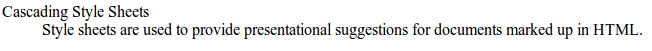
\includegraphics[scale=.5]{definition-list.png}
\end{frame}

\begin{frame}{Images}
 \lstinline!<img>!  Tag 
 \begin{itemize}
  \item \lstinline!<img>! is used to display an image on a page. 
  \item \lstinline!<img>! tag is an empty tag that contains attributes only and do not have  closing tag.
  \item Use the src (Source) attribute i.e., URL  or the path of the image to be displayed.
 \end{itemize}
\end{frame}

\begin{frame}{Images}
 \begin{block}{Example}
  \lstinline!<img  src = ``graphics/talentsprint.gif''>!
 \end{block}
The browser will look for the image name talentsprint.gif in a graphics folder in the same folder where the html document  itself resides.  This is called Relative Path.
\end{frame}

\begin{frame}{Images}
 \begin{block}{Example}
  \lstinline!<img src = ``http://dashboard.talentsprint.com/images/talentsprintlogo.jpg''> !
 \end{block}
In this case it is called Absolute Path. As it doesn't related to the current directory.
\end{frame}

\begin{frame}{Images}
 \lstinline!<img>! Attributes 
 
 \vspace{1pc}
 Image Dimensions
 \begin{itemize}
  \item \textbf{ Height:} Specifies the height of an image in pixels or \%
  \item \textbf{Width:} Specifies the width of an image in pixels or \%
  \item \textbf{Border:}  Specifies the width of the border in terms of pixels around an image.
 \end{itemize}
\end{frame}

\begin{frame}{Images}
 Alignment of Images
 
 \vspace{1pc}
 \textbf{align}
 \begin{itemize}
  \item Specifies the alignment of an image according to surrounding elements
  \item left, right, top, middle, bottom are the values of align attributes
 \end{itemize}
\begin{minipage}{5cm}
 \begin{block}{Example}
 \lstinline!<img src = ``ts.jpg'' align = ``right''>!
 \end{block}
\end{minipage}
\begin{minipage}{5cm}
 
\includegraphics[scale=.5]{image-demo.png}
\end{minipage}
\end{frame}

\begin{frame}{Images}
 Alignment of Images
 \begin{block}{Example}
  \lstinline!<p> This is text in paragraph tag...<img src = ``ts.jpg'' align = ``top''></p>!
 \end{block}
 
\includegraphics[scale=.5]{text-image-right.png}
\end{frame}

\begin{frame}{Images}
 Alignment of Images
 \begin{block}{Example}
  \lstinline!<p> This is text in paragraph tag...<img src = ``ts.jpg'' align = ``bottom''></p>!
 \end{block}
 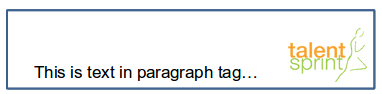
\includegraphics[scale=.5]{text-image-bottom.png}
 
 ``middle'' value can be used similarly
\end{frame}










\begin{frame}{HTML Basics}
 \begin{figure}[H]
 \begin{center}
   
\includegraphics[scale=.3]{qa.png}   
 \end{center}
  \end{figure}
\end{frame}

\end{document}
